\section{Reaching}
\label{sec:reaching}

In this section, we describe two approaches which have been 
implemented on our robot to solve the reaching task. A first method 
uses the forward mapping between the arm joint space and the three 
dimensional position of the hand represented in the head reference 
frame $\begin{bmatrix} \theta_y & \theta_p & \alpha_v^d\end{bmatrix}^\top \in \mathbb R^3$. 
The second method uses a visual servoing technique to control the 
speed of the arm so to minimize the position of the hand in the 
image plane with respect to a desired target (usually the fixated object).

\subsection{Open Loop Reaching}
Suppose the robot is tracking a target using the control strategy described in 
Section \ref{Sec:TrackerController}. In the further assumption of perfect tracking 
(the visual error is zero), the three dimensional spatial position of the target 
with respect to the robot, denoted $\tilde {\mathbf x}_{target} \in \mathbb R^3$, 
is a function of the head configuration $\mathbf q_{head} =
\begin{bmatrix} \theta_y & \theta_p & \theta_r & \alpha_v^d & \alpha_v^c & \alpha_t^c \end{bmatrix}^\top \in \mathbb R^6$.
However, the representation of the target position, $\tilde {\mathbf x}_{target}$, 
in terms of the full head configuration, $\mathbf q_{head}$, is clearly redundant.
Specifically, the same target position can be represented different head configurations. 
In order to obtain a one to one mapping between the target configuration and the 
head position we have to carefully analyze the {\tt tracker controller}. During tracking 
$\theta_r$ is maintained stationary ($\theta_r^d = 0$), while the head controller 
poses additional constraints on the head joints; in particular we know from section 
\ref{Sec:TrackerController} that the controller minimizes $\alpha_t^c$ and
$\alpha^c_v$ (see equation (\ref{Eq:HeadEyeControl})) so that they asymptotically
converge to $\alpha_t^c \rightarrow 0$ and $\alpha_v^c \rightarrow 0$. Ideally, after 
fixation has been achieved, we should have:
%
\begin{eqnarray}
{\mathbf q}_{head}=
\begin{bmatrix} \theta_y & \theta_p & 0 & \alpha_v^d & 0 & 0 \end{bmatrix}^\top \in \mathbb R^6.
\end{eqnarray}
%
Since there exists a one to one mapping between the three dimensional position of the target 
$\tilde {\mathbf x}_{target}$ and the three non-zero variables $\theta_y$, $\theta_p$ 
and $\alpha_v^d$, we can define:
%
\begin{eqnarray}
\mathbf x_{target}=
\begin{bmatrix} \theta_y & \theta_p & \alpha_v^d\end{bmatrix}^\top \in \mathbb R^3.
\end{eqnarray}
%
This new variable $\mathbf x_{target} \in \mathbb R^3$ uniquely codes the position 
of the target. The representation is very similar to a three dimensional polar 
representation in which $\theta_y$ and $\theta_p$ code respectively azimuth 
and elevation, while distance is substituted with $\alpha_v$ (\emph{vergence} angle). 

If the robot is tracking the hand, the same subset of the head joint space can be used to code the spatial location of the hand:
%
\begin{eqnarray*}
\mathbf x_{hand}=
\begin{bmatrix} \theta_y & \theta_p & \alpha_v^d\end{bmatrix}^\top \in \mathbb R^3.
\end{eqnarray*}
%
Under these assumptions we can train a neural network to approximate the forward mapping between the arm joint space $\mathbf q_{arm}$ and the position of the hand $\mathbf x_{hand}$:
%
\begin{equation} 
\label{Eq:forward}
\mathbf x_{hand}=f_{arm}(\mathbf q_{arm}), \qquad f_{arm} : \mathbb R^3 \longrightarrow \mathbb R^4.\end{equation}
%
Suppose now that we want to control the robot to reach for a target it is currently 
fixated. Formally the problem can be formulated as determining the value of $\mathbf q_{arm}$ 
which solves the following minimization:
%
\begin{equation} 
\label{Eq:reaching1}
  \displaystyle\min_{\mathbf q_{arm}}\left(J\right)=\displaystyle\min_{\mathbf q_{arm}}
  \left\|\mathbf x_{hand} - \mathbf x_{target}\right\|^2,
\end{equation}
%
where $\mathbf x_{target}$ is measured from the encoders of the head, while 
$\mathbf x_{hand}$ is computed from $\mathbf q_{arm}$ through Eq. (\ref{Eq:forward}). Given the 
redundancy of the arm kinematics the minimization (\ref{Eq:reaching1}) has infinite solutions. To 
overcome this problem we constrained the solution so that one of the joint, for example 
joint number 2, is forced to remain as close as possible to a predefined position $q_{20}$:
%
\begin{equation} 
\label{Eq:reaching2}
  \displaystyle\min_{\mathbf q_{arm}}\left(J_c\right)=\displaystyle\min_{\mathbf q_{arm}}
  \left[
  \left\|\mathbf x_{hand} - \mathbf x_{target}\right\|^2 + \left(q_{arm,2}-q_{20}\right)^2
  \right].
\end{equation}

The numerical optimization of (\ref{Eq:reaching2}) can be performed with different 
numerical tools. Discussing the different properties of these numerical tools falls 
outside the scope of this paper. In our implementation, we used the downhill simplex 
method \cite{ne:Computer:65} as implemented in \cite{mo:Press:90}.

To learn the forward map of equation (\ref{Eq:forward}) we programmed the robot 
to perform random movement with the arm (chosen to uniformly sample 
a predefined region in the robot workspace). During this ``exploratory'' phase the robot
tracked the hand, to collect samples of the form:
%
\begin{center}
\begin{math}
  \left(\begin{array}{cc}
    \mathbf x_{hand} & \mathbf q_{arm} \end{array}\right)_{0,1\dots,k}
\end{math}
\end{center}
%
A neural network was then trained to learn the relation:
%
\begin{center} 
\begin{math}
  \mathbf x_{hand}=\hat{f}_{arm}\left(\mathbf q_{arm}\right)
\end{math}
\end{center}
%
which approximates equation (\ref{Eq:forward}).

\begin{figure}[tbp]
\centerline{
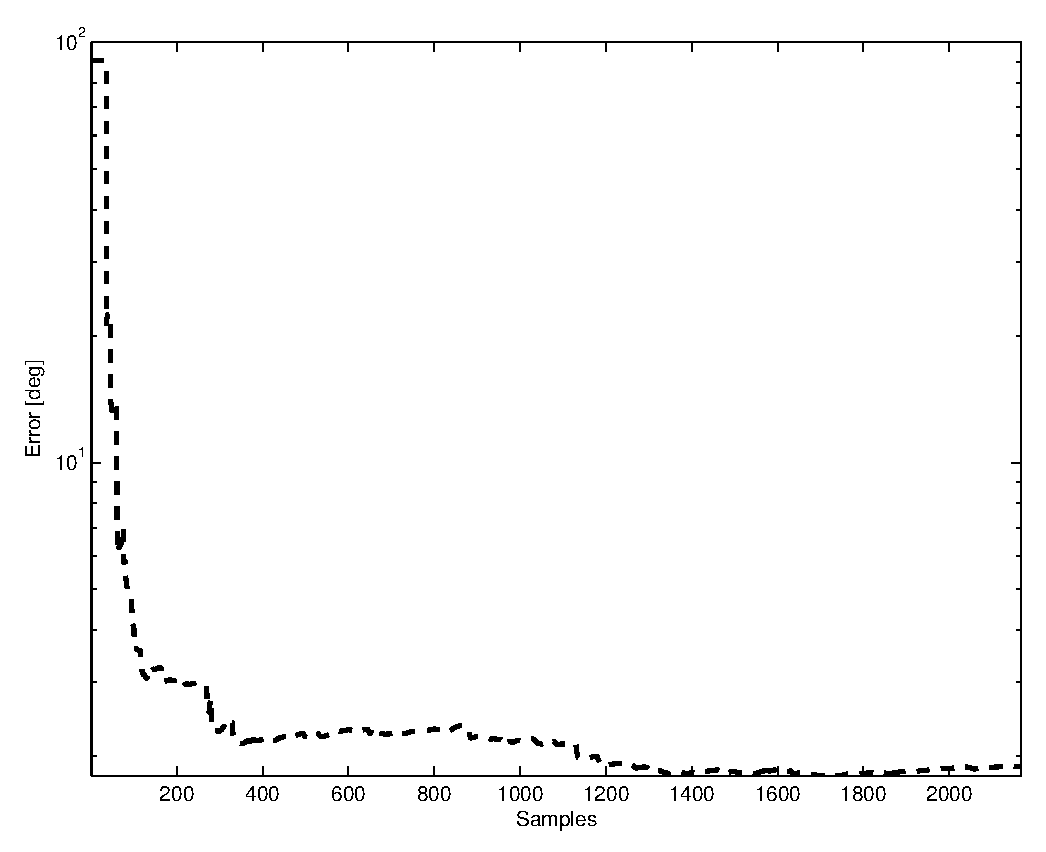
\includegraphics[width=4.0in, angle=0 ]{./Figure/reachingError1.eps}
} \caption{Error.} 
\label{fig:Reaching error}
\end{figure}



























